\chapter{The effect of encryption} \label{effect of encryption}

This chapter includes analysis on how adding encryption to a backend-application affects its complexity and performance.
The analysis is based on the POC project built for the thesis.

\section{The effect on complexity}

Adding extra features to any application obviously increases the complexity.
This complexity adds to the cost of maintaining the application, as the codebase gets larger and therefore harder to reason about.
There are options for dealing with the complexity, such as building abstractions that make reasoning with the program code on a higher level easier.
\cite{complexity-triggers}

\subsection{The effect on the complexity of the program code}

Adding envelope encryption to the program code and encrypting the database columns increases the complexity of the application.
Node.js’ crypto-module handles most of the encryption work, but interfacing with the Cloud Key Management is done using Google’s pre-made Npm-library which adds a dependency to manage.
A bit of additional configuration is required for accessing the GCP project as well as storing cryptographic secrets.

In the implemented POC project, the main encryption logic is abstracted into the \texttt{encryption.ts}-file, into only 6 functions.
This is quite a small amount of code to implement the encryption, which makes it easier to understand and maintain.
However, it still adds to the overall complexity of the application.

The design of the POC calls the encrypt and decrypt functions right at the service-level before or after accessing the database respectively.
The functions are called only on the sensitive fields, and not on database identifiers for example.
An example of this is shown in Listing \ref{alg:encrypt-appointment}.
This logic is not very complex, as the encryption itself is not implemented here, but it still requires adding quite a large amount of code.
The POC has no generic solution for encrypting any object, so an encrypt and decrypt function have to be created for each data type separately.

\subsection{The effect on the complexity of the infrastructure}

The addition of envelope encryption and storing the secrets required also increases the requirements of the infrastructure.
The two new Google Cloud services added are Cloud Key Management and Secret Manager.
Both of these also require IAM-configuration to allow our application to access them.

Cloud Key Management is a fully managed service, and not much configuration is required from the developer.
However, being an external API, it adds a possibility for an I/O bottleneck in our application.
This is why the POC application uses envelope encryption, only wrapping the key encryption key with the KMS.
Google Cloud’s documentation also suggests doing this. \cite{googlecloud}
The request-based pricing of KMS is also something that might affect very large applications.
Rotating the KMS keys is also something not implemented in the POC, which should be taken care of in a real world application.

Service Manager is another fully managed service which requires just as little configuration.
Only the secret, its data and IAM-configuration for the application are required.
Referencing the secrets in Cloud Run’s configuration is not a lot of added code either.
From the application’s point of view, it does not change anything where the environment variables are stored: the application accesses them the same way in either case.

\section{The effect on performance}

In this section, the fully built application's performance is tested.
The performance of the application is tested with both encryption enabled and disabled.
The goal is to measure the overhead caused by the encryption.

\subsection{Load testing}

Load testing refers to the practice of measuring a web application's quality of service performance.
The quality of service consists of two measures:
\begin{itemize}
    \item 
    \textit{Availability} – the percentage of times a customer is able to access the application
    \item 
    \textit{Response time} – the time it takes for the customer's action to be fulfilled.
\end{itemize}
Load testing from a single geographical location and during a single time window will not give you the complete picture.
End-to-end response time is dependent on a variety of things such as the user's location and the type of their network connection.
\cite{loadtesting}

Load testing can be used to predict a web application's performance at specific loads.
The load testing data can be further analysed to calculate the throughput of an application.
The throughput is a function of the number of concurrent requests and the stress on the system resources, most easily measured in request time.
\cite{loadtesting}

\subsection{The testing strategy}

To load test the POC application, we will first limit the scaling on the Cloud Run service to a maximum of one container.
This is done to observe changes in the stress level without needing equally as scalable tooling for running the load tests.
2000 simultaneous requests is enough to observe a difference in the performance of the application.
Under default settings, Cloud Run would activate more than 50 containers to support the load.

The testing will be conducted with Apache's JMeter: an application designed to load test and measure performance of many different applications/protocols.\footnote{Homepage of Apache JMeter: https://jmeter.apache.org/}
JMeter is configured to run 2000 simultaneous requests to the server and measure the response times.
The application is first built and deployed with encryption disabled, and then with encryption enabled.
Before each test, the database is cleared.
The test plan is to first call the \texttt{POST /practitioners/} endpoint 2000 times, adding the number of practitioners in to the database.
Second, we will call the \texttt{GET /practitioners/} endpoint 2000 times, fetching all of the practitioners each time.
Hypothesis for the results is that the added computation required by the encryption will cause an increase in response time and therefore a decrease in throughput.

\subsection{The results of the load testing}

The load test on the \texttt{POST /practitioners/} endpoint show a clear difference in both response time and throughput.
When encryption is enabled, the server takes almost a second longer to respond to begin with, and only slows from there.
While unencrypted, the response time does climb as the load increases, but the throughput still manages to go quite high before plateauing.
Both tests succeeded in all of the requests, so 100\% availability was achieved.
The visualization of the tests results is shown in Figure \ref{fig:post-practitioners}.

\begin{figure}[!htb]
\centering
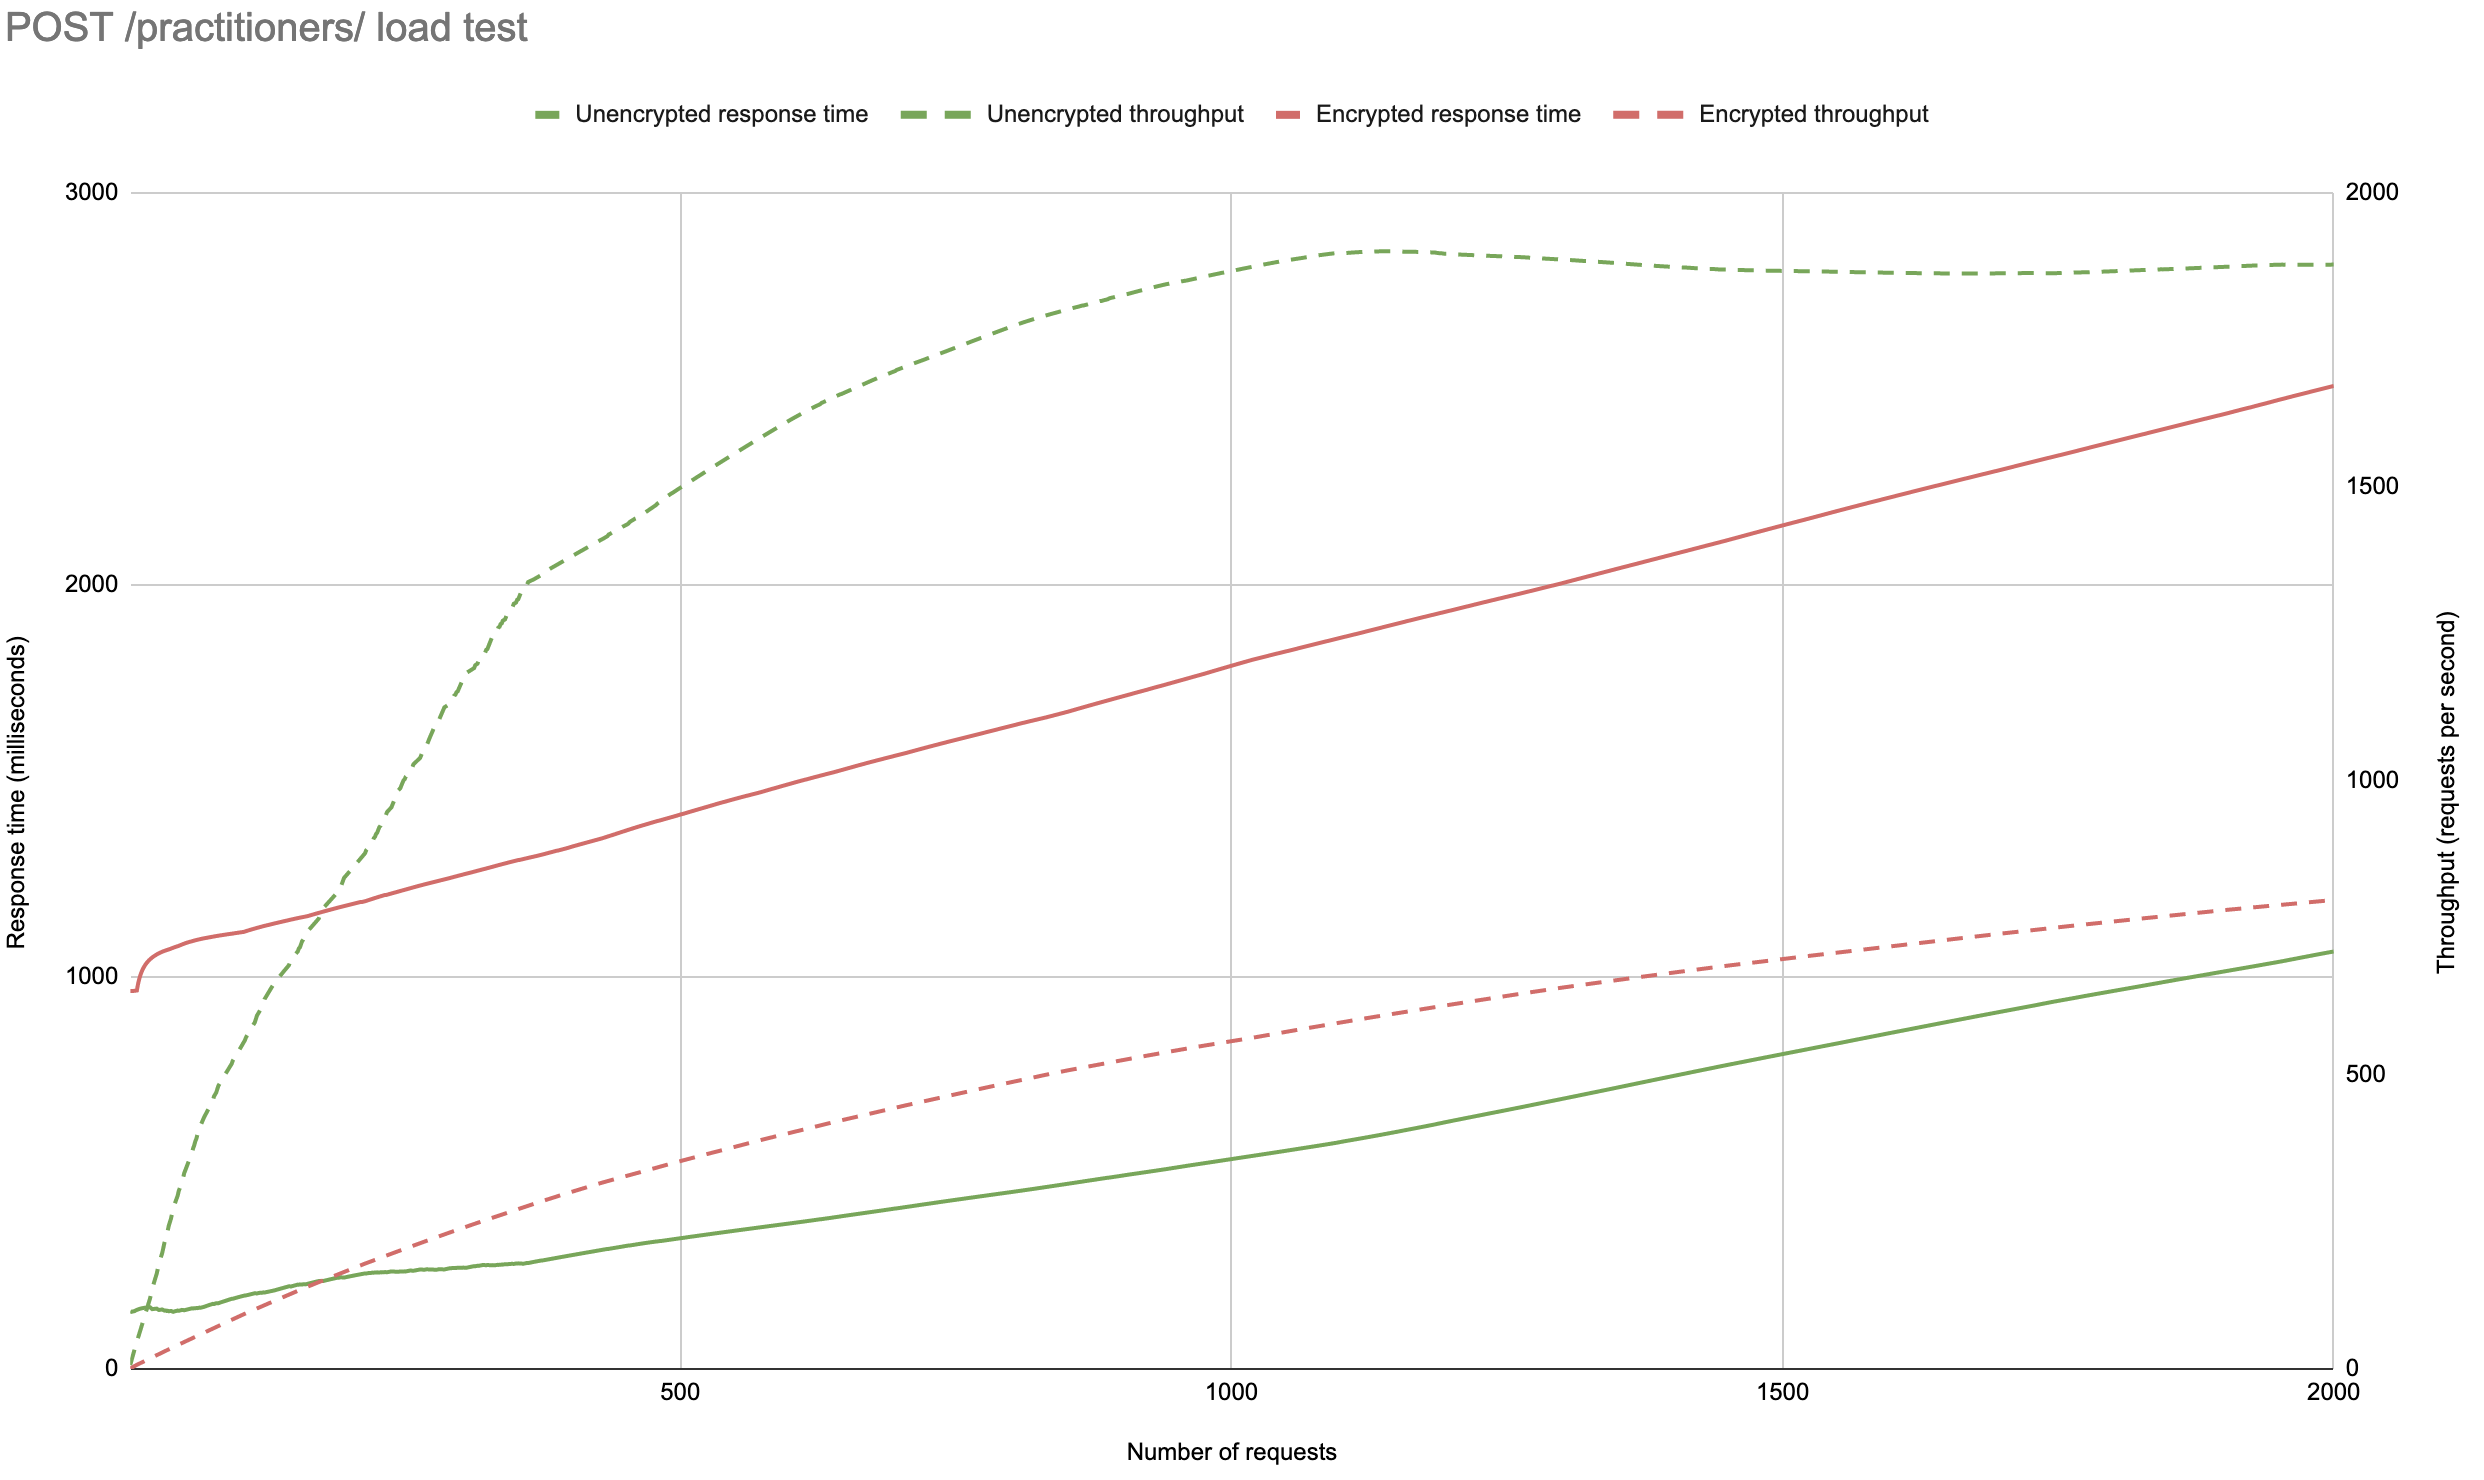
\includegraphics[scale=0.35]{post-practitioners}
\caption{POST /practitioners/ load test results.}
\label{fig:post-practitioners}
\end{figure}

The load tests on the \texttt{GET /practitioners/} endpoint show quite a different result.
At first, both encrypted and unencrypted take approximately the same time to respond to the request.
Both of the response times start climbing as the load increases, the encrypted response time spiking very sharply.
However, both of the response times plateau after enough load.
The encrypted application's response time plateauing around a hundred requests, and the unencrypted application's at around 500 requests.
This causes the throughput to start climbing instead.
The visualiztion of the tests results is shown in Figure \ref{fig:get-practitioners}.

\begin{figure}[!htb]
\centering
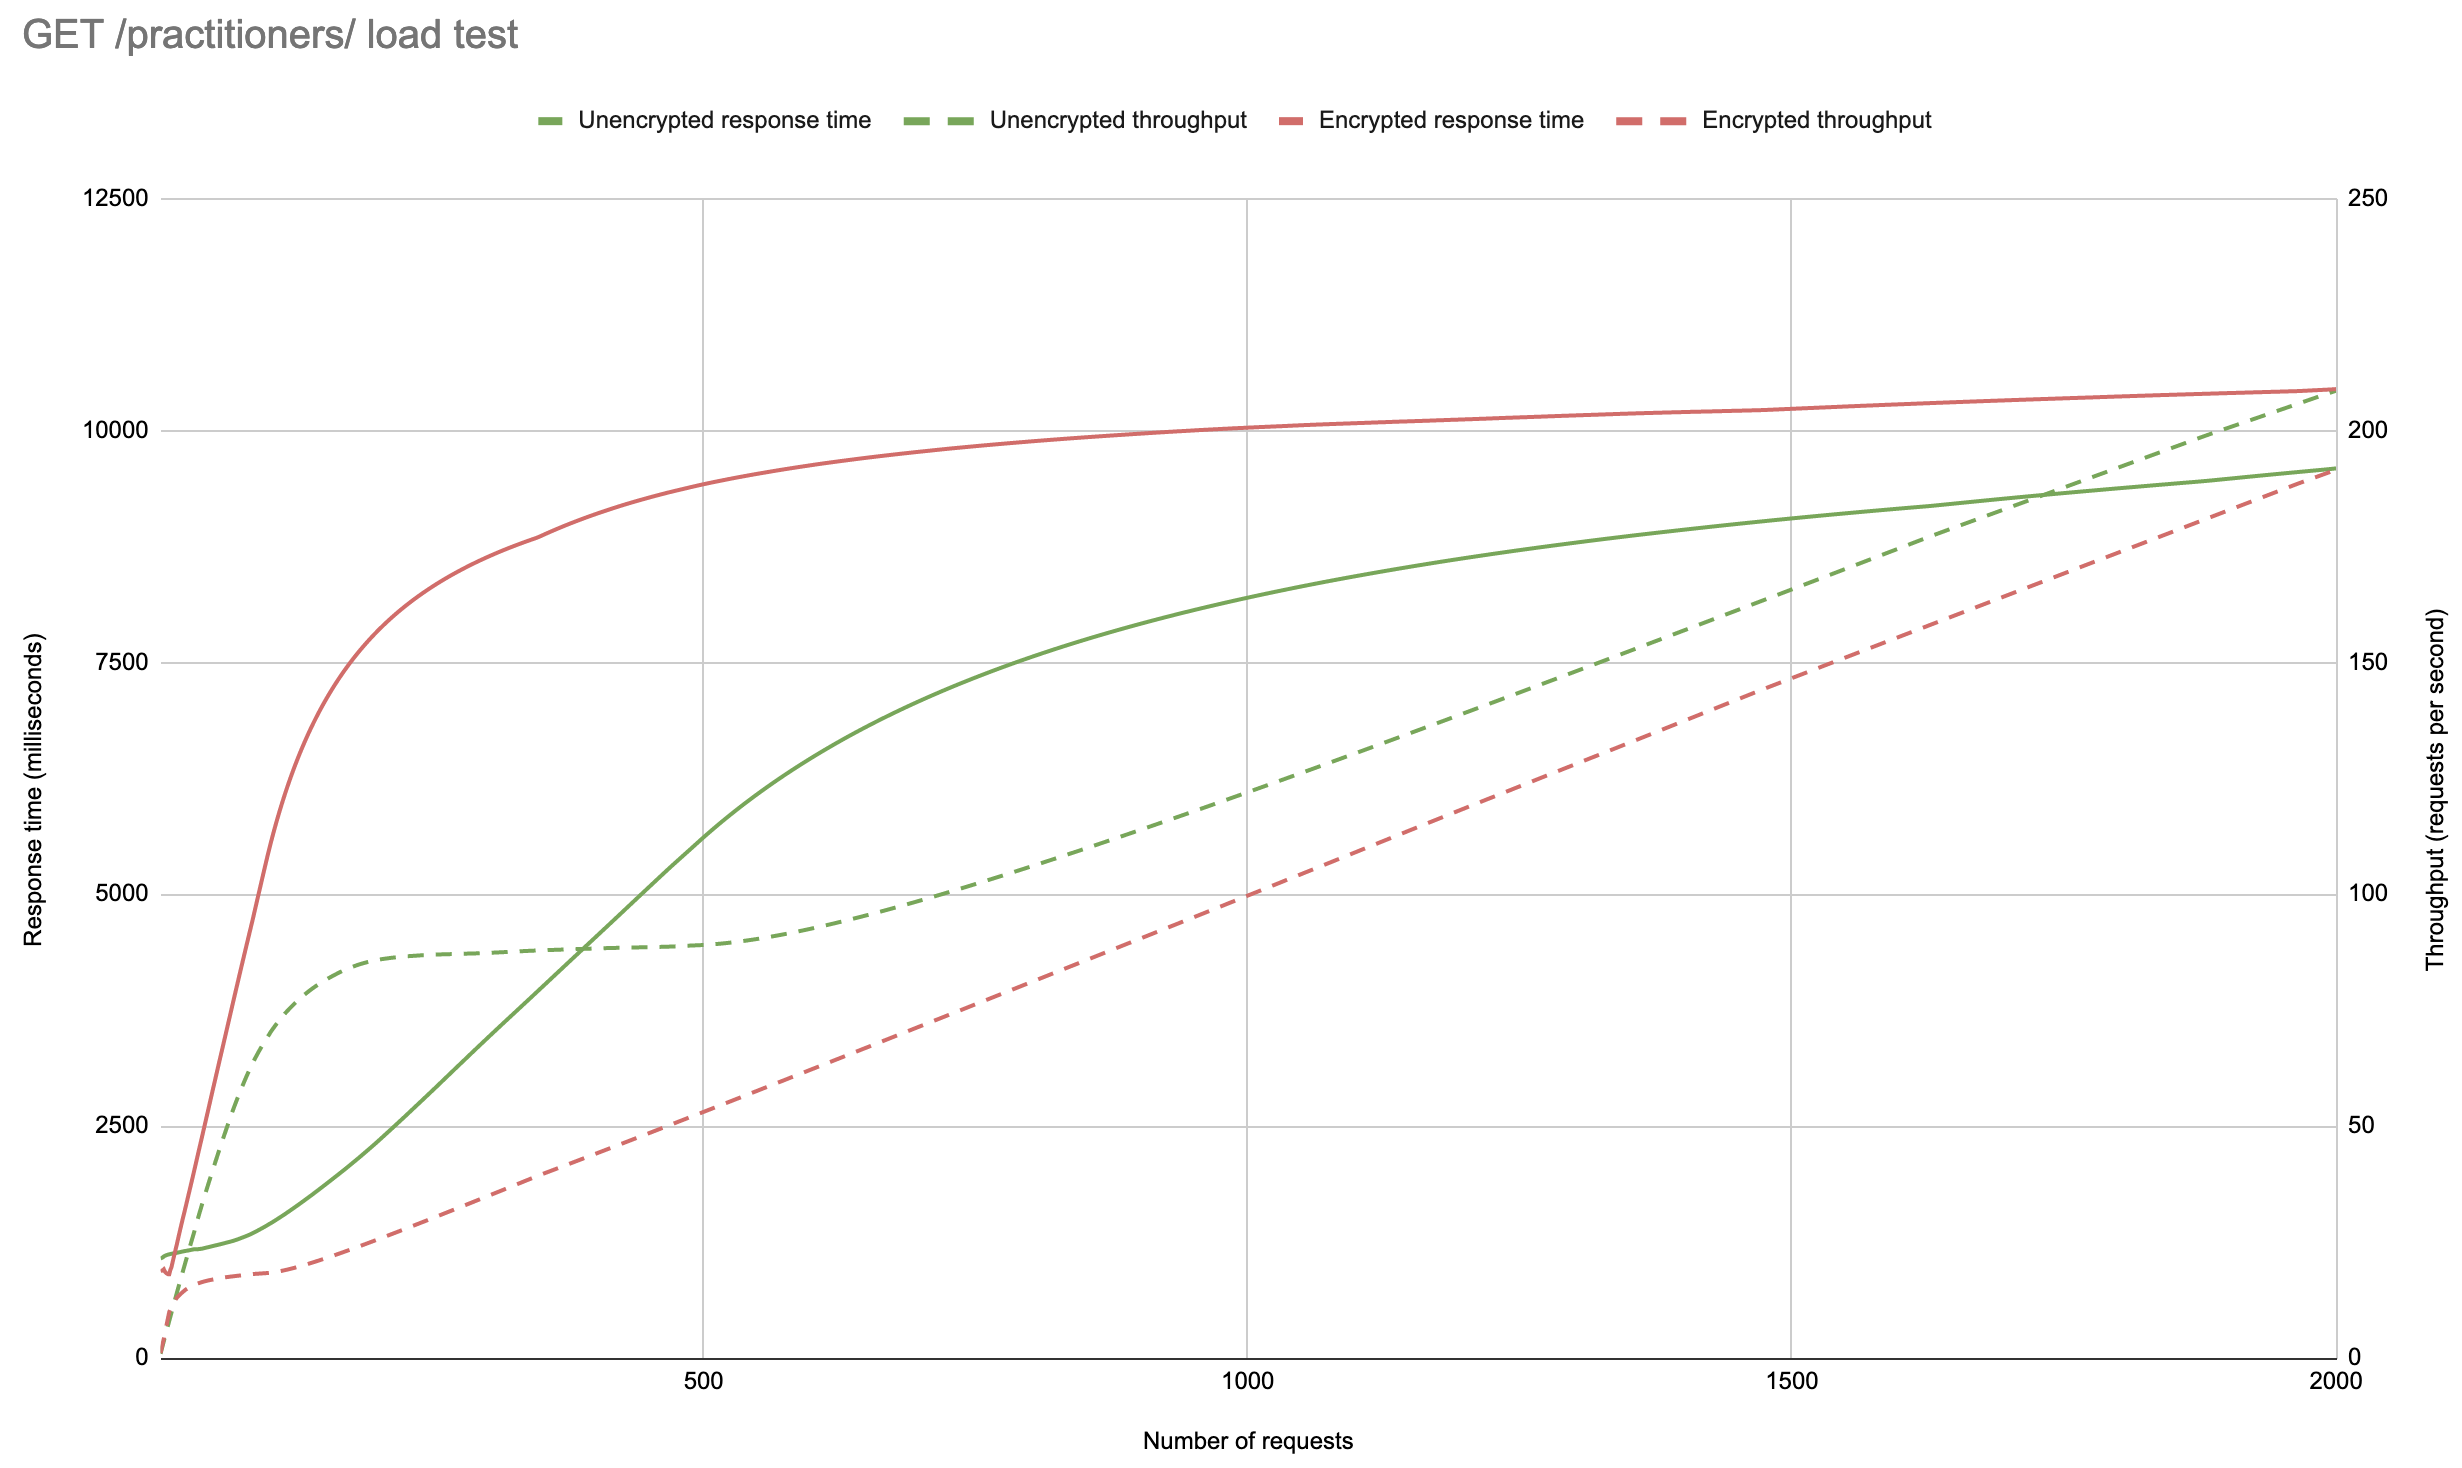
\includegraphics[scale=0.35]{get-practitioners}
\caption{GET /practitioners/ load test results.}
\label{fig:get-practitioners}
\end{figure}

The reason for the odd results for the \texttt{GET /practitioners/} endpoint is the success rate of the requests: the server starts refusing requests after enough load and responding with \texttt{HTTP 429 Too Many Requests} instead.
This means our application was not able to serve the load of 2000 simultaneous requests with 100\% availability.
The number of errors increasing as load increases is visualized in Figure \ref{fig:get-practitioners-errors}.

\begin{figure}[!htb]
\centering
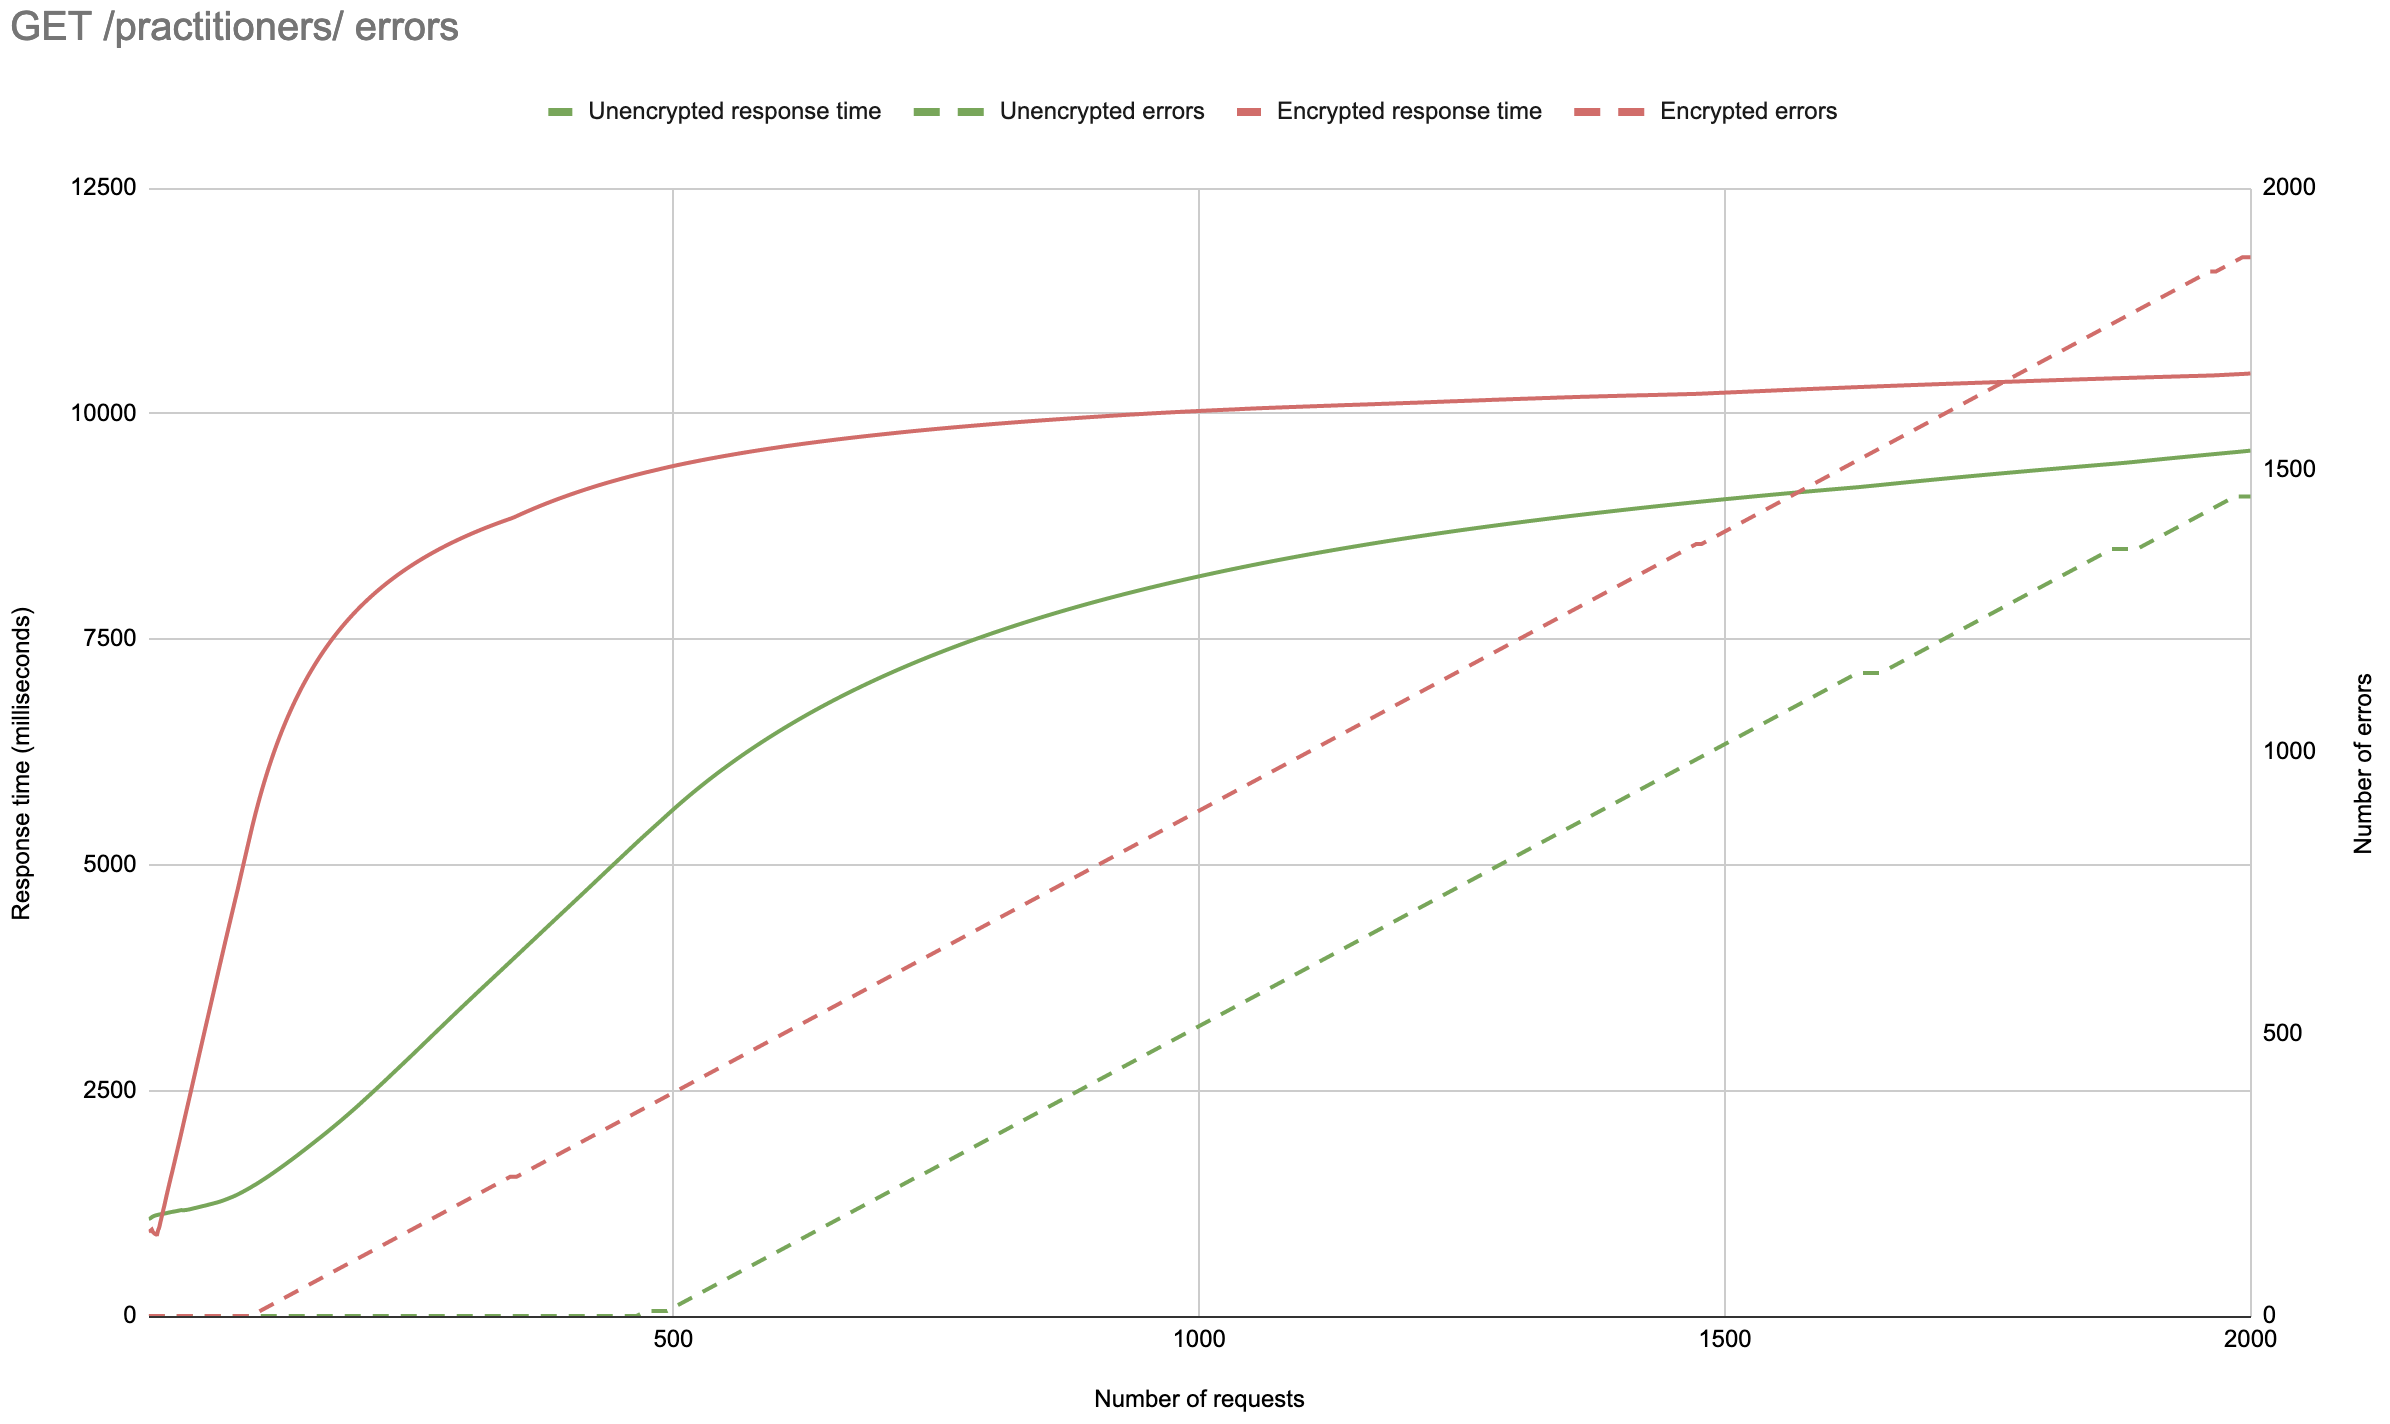
\includegraphics[scale=0.35]{get-practitioners-errors}
\caption{GET /practitioners/ response time and errors.}
\label{fig:get-practitioners-errors}
\end{figure}

The difference in the two endpoints' load tests is most likely caused by the large difference in the work required by each endpoint.
Namely, the amount of data passing through the application.
In the case of the \texttt{POST /practitioners/} endpoint, a single practitioner-object is sent to the server and stored in the database.
As for the \texttt{GET /practitioners/} endpoint, all of the practitioner-objects in the database have to be queried from the database and converted into JSON.

\section{Analysis}

The addition of encryption and its requirements on the infrastructure adds to the complexity of the application.
This added complexity will increase the cost of building and maintaining a similar application.
However, that complexity is largely dealt with by existing solutions available, such as the Cloud Key Management and Node.js' crypto-module used here.
No low-level knowledge of implementing cryptography is required by the developer, only enough to use the existing solutions securely.
Due to the laws in effect in Finland requiring proper security measures from all applications dealing with sensitive data, the added cost of this extra complexity should be taken into account when budgeting for such a project.

The hypothesis of encryption affecting performance negatively holds true.
However, the difference is not as large as expected.
Modern hardware is excellent at running encryption, and our application is most likely limited more by its I/O, rather than the extra computation required by the encryption.

The \texttt{GET /practitioners/} endpoint failing after some requests is not because of the encryption, as the unencrypted test was also affected by this.
The endpoint's functionality of loading an entire database table's data and sending it to the client is not a common real world use case.
Calling such an endpoint thousands of times simultaneously is certainly not a realistic scenario.

The POC project implemented leaves room for improvement in all of the fields tested.
Options for improving the design and implementation are discussed in the next chapter.
